% Provenance (never printed): see sources/outline_sources.md (Year 3: rift
% models, normal-fault systems, metamorphic core complexes, strike-slip
% systems). Brief: sources/book5/BRIEFS.md, ch. 9. Curves from
% figdata/bachelor-3/domino_extension.py and rollover.py. Exercise and problem
% values in the Book 5 scratch calculator calc/ch09.py.
\chapter{伸展与走滑构造}\label{ch:b3:extension-strike-slip}

在塞拉内华达山脉与科罗拉多高原之间，山脉与盆地
相间排列，宛如田垄；每座山脉都是沿正断层倾斜的
地壳块体。在其中一些山脉的核部，岩石
曾埋藏于 23 至 \qty{30}{km} 深处、温度为 500 至 \qty{650}{\celsius}，如今出露于地表，
位于一条倾角仅几度的单一断层之下。大陆可被拉伸至两倍或更多，
并沿断层横向撕裂，这些断层弯曲、呈台阶状，
并张开深达 \qty{10}{km} 的盆地。本章建立
伸展与走滑断层的几何学、支配二者的少数规律，
以及真实构造系统留下的证据。
% ledger: cooper10:snake-range, mcq05:basin-range, tb93:dead-sea-basin

\begin{recall}
正断层、走滑断层与转换断层、半地堑及大陆
裂谷见本科一年级分册中关于裂谷以及断层、褶皱与构造组构的章节，
其中包括安德森理论：当 $\sigma_1$ 竖直时，正断层
的倾角为 $\ang{45} + \phi/2$，约 \ang{60}；当 $\sigma_2$ 竖直时，走滑断层
的走向以 $\ang{45} - \phi/2$ 偏离 $\sigma_1$。岩石摩擦的拜尔利
定律为 $\tau = 0.85\,\sigma_n$（低于 \qty{200}{MPa} 时），而 $\tau =
\qty{50}{MPa} + 0.6\,\sigma_n$（高于此值时），见其中关于应力、应变与流变学的一章。
拉伸模型（岩石圈按均匀系数 $\beta$ 减薄）与裂谷盆地，
见本科二年级分册中比较沉积盆地的章节。
\omterm{def:b3:deformation-mechanisms:shear-zone}{剪切带}与糜棱岩见
\cref{ch:b3:deformation-mechanisms}；\omterm{def:b3:extension-strike-slip:detachment}{拆离断层}的深度可由过剩面积
$A = Sh$ 求得，见\cref{ch:b3:structural-analysis}。
\end{recall}
% ledger: byerlee:1975

\section{裂谷的两种模型}\label{sec:b3:extension-strike-slip:models}

本科二年级分册中的拉伸模型认为，同一位置的整个岩石圈
按相同系数减薄：地壳与地幔一起、对称地、以纯剪切方式减薄。
许多裂陷边缘并不对称：一侧是宽阔的倾斜块体区，
另一侧为狭窄陡峭的斜坡，地幔减薄区位于地壳减薄区
的旁侧，而非其下方。

\begin{definition}[简单剪切裂谷模型]\label{def:b3:extension-strike-slip:rift-models}
在\emph{简单剪切裂谷模型}\index{简单剪切裂谷模型}中，岩石圈
沿一条低角度\omterm{def:b3:deformation-mechanisms:shear-zone}{剪切带}被拉开，该\omterm{def:b3:deformation-mechanisms:shear-zone}{剪切带}自地表
切至岩石圈底部。位于\omterm{def:b3:deformation-mechanisms:shear-zone}{剪切带}之上的板块，即上部板块，
失去其下部；位于其下的板块，即下部板块，
被从其下方拉出。地壳的减薄与地幔的减薄
在水平方向上相互错开，大陆破裂时形成的两个共轭边缘
是不对称的。
\end{definition}

真实的裂谷兼具二者：上地壳发生脆性断层作用，
下方发生韧性减薄，地幔的减薄范围可能比地壳更宽或更窄，
即深度相关的伸展。热地幔在裂谷之下上涌时，
或在简单剪切情形下于其侧翼之下上涌时，浮力抬升裂谷的肩部，
使其高出盆地底面成为山脉。

\begin{omfigure}
\begin{tikzpicture}[scale=0.95, >=stealth]
% (a) pure shear
\begin{scope}
\fill[omLithBasalt!40] (0,-3.2) rectangle (6.6,-1.3);
\fill[omLithGranite!50] (0,0) -- (2.2,0) -- (2.5,-0.35) -- (4.1,-0.35) -- (4.4,0) -- (6.6,0) -- (6.6,-1.3)
  -- (4.4,-1.3) -- (3.3,-0.95) -- (2.2,-1.3) -- (0,-1.3) -- cycle;
\fill[omLithBasalt!40] (2.2,-1.3) -- (3.3,-0.95) -- (4.4,-1.3) -- cycle;
\fill[orange!25] (0,-3.2) -- (1.8,-3.2) -- (3.3,-2.1) -- (4.8,-3.2) -- (6.6,-3.2) -- (6.6,-3.7) -- (0,-3.7) -- cycle;
\draw (0,0) -- (2.2,0) -- (2.5,-0.35) -- (4.1,-0.35) -- (4.4,0) -- (6.6,0);
\draw (0,-1.3) -- (2.2,-1.3) -- (3.3,-0.95) -- (4.4,-1.3) -- (6.6,-1.3);
\draw (0,-3.2) -- (1.8,-3.2) -- (3.3,-2.1) -- (4.8,-3.2) -- (6.6,-3.2);
\draw[thick] (2.2,0) -- (2.75,-0.85); \draw[thick] (4.4,0) -- (3.85,-0.85);
\node[font=\scriptsize] at (0.7,-0.65) {地壳};
\node[font=\scriptsize, align=center] at (0.9,-2.25) {地幔 \\岩石圈};
\node[font=\scriptsize] at (1.2,-3.48) {软流圈};
\draw[<-] (-0.1,0.25) -- (0.6,0.25); \draw[->] (6.0,0.25) -- (6.7,0.25);
\node[font=\small] at (3.3,-4.2) {(a) 纯剪切};
\end{scope}
% (b) simple shear: crust thinned near the breakaway (left), mantle beneath the upper plate (right)
\begin{scope}[xshift=7.4cm]
\fill[omLithBasalt!40] (0,-3.2) rectangle (6.6,-1.3);
\fill[omLithGranite!50] (0,0) -- (0.9,0) -- (1.2,-0.3) -- (2.2,-0.3) -- (2.5,0) -- (4.0,0)
  .. controls (4.6,0.18) and (5.2,0.18) .. (5.8,0) -- (6.6,0) -- (6.6,-1.3)
  -- (2.9,-1.3) -- (2.0,-0.7) -- (1.2,-1.3) -- (0,-1.3) -- cycle;
\fill[omLithBasalt!40] (1.2,-1.3) -- (2.0,-0.7) -- (2.9,-1.3) -- cycle;
\fill[orange!25] (0,-3.2) -- (3.4,-3.2) -- (4.8,-2.1) -- (6.0,-3.2) -- (6.6,-3.2) -- (6.6,-3.7) -- (0,-3.7) -- cycle;
\draw (0,0) -- (0.9,0) -- (1.2,-0.3) -- (2.2,-0.3) -- (2.5,0) -- (4.0,0)
  .. controls (4.6,0.18) and (5.2,0.18) .. (5.8,0) -- (6.6,0);
\draw (0,-1.3) -- (1.2,-1.3) -- (2.0,-0.7) -- (2.9,-1.3) -- (6.6,-1.3);
\draw (0,-3.2) -- (3.4,-3.2) -- (4.8,-2.1) -- (6.0,-3.2) -- (6.6,-3.2);
\draw[omThm, very thick] (0.9,0) .. controls (2.4,-0.9) and (3.9,-1.8) .. (5.4,-3.2);
\node[font=\scriptsize, align=center] at (5.0,-0.6) {上部板块};
\node[font=\scriptsize, align=center] at (1.3,-2.3) {下部板块};
\node[omThm, font=\scriptsize, align=center] at (3.0,-2.15) {剪切 \\带};
\node[font=\scriptsize, align=center] at (4.9,0.42) {抬升侧翼};
\draw[<-] (-0.1,0.25) -- (0.6,0.25); \draw[->] (6.0,0.25) -- (6.7,0.25);
\node[font=\small] at (3.3,-4.2) {(b) 简单剪切};
\end{scope}
\end{tikzpicture}

\par\smallskip{\small 两种端元裂谷模型（未按比例绘制）。(a) 纯
剪切：地壳与地幔岩石圈在裂谷下方一同减薄，两侧均发育
正断层。(b) 简单剪切：一条低角度\omterm{def:b3:deformation-mechanisms:shear-zone}{剪切带}穿过
岩石圈；地壳在其地表迹线附近减薄，地幔在
远侧、上部板块之下减薄，因此裂谷不对称，其
位于减薄地幔之上的侧翼被抬升。}\label{fig:b3:extension-strike-slip:models}
\end{omfigure}

\section{正断层系统}\label{sec:b3:extension-strike-slip:faults}

\begin{definition}[多米诺断层作用]\label{def:b3:extension-strike-slip:domino}
在\emph{多米诺断层作用}\index{多米诺断层作用}中，一组平行的平面
正断层将上地壳切割成刚性块体，随着区域伸展，
这些块体一同转动，宛如一排倒下的书：断层变得
愈发平缓，原本水平的岩层则向相反方向倾斜。
\end{definition}

\begin{theorem}[多米诺式伸展]\label{thm:b3:extension-strike-slip:domino}
设以平行平面断层为界的刚性块体，断层原先倾角为
$\theta_0$，块体旋转至断层倾角为 $\theta$。此时岩层倾角为 $\theta_0
- \theta$，倾向背离断层，区域的伸展
因子为
\[
  \beta = \frac{\sin\theta_0}{\sin\theta} .
\]
\end{theorem}

\begin{proof}
块体是刚性的，因此两相邻断层之间的垂直距离 $d$
保持不变。沿水平线，两平行平面倾角为 $\theta$、间距为 $d$，
截得一段长度为 $d/\sin
\theta$ 的线段；区域宽度与该线段长度成正比，由
$d/\sin\theta_0$ 变为 $d/\sin\theta$。块体旋转的角度为
断层变缓的角度 $\theta_0 - \theta$，原先水平的
岩层随之一起转动。
\end{proof}

仅靠旋转所得的伸展较小：起始倾角为 \ang{60} 的断层
变缓至 \ang{30}，使区域伸展 $\beta = 1.73$。旋转不会无限进行，
断层越缓越难错动：竖直的
$\sigma_1$ 对断层的压力增大，而剪切作用减弱。

\begin{proposition}[正断层的摩擦锁定]\label{prop:b3:extension-strike-slip:lockup}
设无黏聚力的断层，摩擦系数为 $\mu$，
以 $t$ 记其与 $\sigma_1$ 所成的角，所有应力均为有效应力。断层在主应力之比
达到下式时发生错动：
\[
  \frac{\sigma_1}{\sigma_3} = \frac{1 + \mu\cot t}{1 - \mu\tan t} ,
\]
该比值的最小值为 $(\sqrt{1 + \mu^2} + \mu)^2$，在 $\tan2t = 1/\mu$ 时取得，
当 $\tan t = 1/\mu$ 时趋于无穷大。若 $\sigma_1$ 竖直，则断层倾角为
$\ang{90} - t$：倾角小于 $\arctan\mu$ 的正断层
完全不能错动。
\end{proposition}

\begin{proof}
记 $m = (\sigma_1 + \sigma_3)/2$，$s = (\sigma_1 - \sigma_3)/2$。在断层面上，
$\sigma_n = \sigma_1\sin^2t + \sigma_3\cos^2t = m - s\cos2t$，
$\tau = (\sigma_1 - \sigma_3)\sin t\cos t = s\sin2t$。错动要求 $\tau =
\mu\sigma_n$；两边除以 $\sigma_3\sin t\cos t$，并整理出 $\sigma_1$，
即得比值，其分母在 $\tan t = 1/\mu$ 时为零。另一种形式中，条件为
$s(\sin2t + \mu\cos2t) = \mu m$。括号内的值至多为
$\sqrt{1 + \mu^2}$，在 $\tan2t = 1/\mu$ 时取得，此时错动所需的
最小比值 $s/m = \mu/\sqrt{1 + \mu^2}$；于是 $\sigma_1/\sigma_3 = (m + s)/(m - s) =
(\sqrt{1 + \mu^2} + \mu)/(\sqrt{1 + \mu^2} - \mu) = (\sqrt{1 + \mu^2} +
\mu)^2$，因为最后两个括号之积为 1。
\end{proof}

取拜尔利的 $\mu = 0.6$，最有利取向的正断层倾角为 \ang{60.5}，
在 $\sigma_1 = 3.12\,\sigma_3$ 时错动；倾角为 \ang{45} 的断层需要 $4.0$，
倾角小于 \ang{31} 的断层均不能错动；取 $\mu = 0.85$ 时，锁定倾角为
\ang{40}。下图给出了这两项结果。当一组多米诺接近锁定时，
会有一组新的陡断层切割旧的一组：高度伸展的区域
通常显示多代断层。

\begin{omfigure}
\begin{tikzpicture}
\begin{groupplot}[group style={group size=2 by 1, horizontal sep=1.6cm},
  omrecord, width=0.47\linewidth, height=0.42\linewidth, title style={font=\small},
  legend style={font=\scriptsize, legend cell align=left}]
\nextgroupplot[title={(a) 刚性多米诺的伸展}, xlabel={现今断层倾角 $\theta$ (\unit{\degree})},
  ylabel={伸展因子 $\beta$}, xmin=10, xmax=70, ymin=1, ymax=4,
  legend style={at={(0.97,0.97)}, anchor=north east}]
% computed in figdata/bachelor-3/domino_extension.py
\addplot[omDef, thick] table[x=dip, y=b70] {figdata/out/bachelor-3-domino_extension-beta.dat};
\addlegendentry{$\theta_0 = \ang{70}$}
\addplot[red!70!black, thick, densely dashed] table[x=dip, y=b60] {figdata/out/bachelor-3-domino_extension-beta.dat};
\addlegendentry{$\theta_0 = \ang{60}$}
\addplot[black, thick, densely dotted] table[x=dip, y=b45] {figdata/out/bachelor-3-domino_extension-beta.dat};
\addlegendentry{$\theta_0 = \ang{45}$}
\nextgroupplot[title={(b) 错动所需的应力比}, xlabel={断层倾角 (\unit{\degree})},
  ylabel={$\sigma_1/\sigma_3$}, xmin=20, xmax=90, ymode=log, ymin=1, ymax=40,
  log ticks with fixed point, ytick={1,2,5,10,20,40},
  legend style={at={(0.97,0.97)}, anchor=north east}]
\addplot[omDef, thick] table[x=dip, y=r060] {figdata/out/bachelor-3-domino_extension-lockup.dat};
\addlegendentry{$\mu = 0.6$}
\addplot[red!70!black, thick, densely dashed] table[x=dip, y=r085] {figdata/out/bachelor-3-domino_extension-lockup.dat};
\addlegendentry{$\mu = 0.85$}
\end{groupplot}
\end{tikzpicture}

\par\smallskip{\small (a) 刚性多米诺区域的伸展因子，其断层由
初始倾角 $\theta_0$ 旋转至 $\theta$。(b) 给定倾角的正断层发生错动
所需的有效主应力之比，
在竖直的 $\sigma_1$ 下，取拜尔利的两个摩擦系数：最小值
出现在约 \ang{60} 与 \ang{65} 附近，锁定倾角 \ang{31} 与
\ang{40} 处为无穷大。}\label{fig:b3:extension-strike-slip:domino}
\end{omfigure}

许多大型正断层是弯曲的：地表附近陡峭，向深部
逐渐变缓，近乎水平地转为一条断层或\omterm{def:b3:deformation-mechanisms:shear-zone}{剪切带}。

\begin{definition}[拆离断层、铲形断层与滚动背斜]\label{def:b3:extension-strike-slip:detachment}
\emph{拆离断层}\index{拆离断层}是一种低角度正断层
或\omterm{def:b3:deformation-mechanisms:shear-zone}{剪切带}，位移很大，可达数千米至数十千米，它将伸展的上盘
与变形方式不同的下盘分隔开。
\emph{铲形断层}\index{铲形断层}是倾角随深度减小的正断层，
其剖面向上凹。铲形断层的上盘
向下、远离断层运动时，为保持与断层接触而发生弯曲：
其岩层向断层倾斜，形成一个宽缓的褶皱，即
\emph{滚动背斜}\index{滚动背斜}。
\end{definition}

\begin{method}[等水平断距作图法]\label{met:b3:extension-strike-slip:heave}
在平行于滑动方向的剖面上，画出\omterm{def:b3:extension-strike-slip:detachment}{铲形断层}上盘经过水平位移
$H$（即水平断距）后的位置：
\begin{enumerate}
  \item 将上盘划分为竖直的柱体。将每个柱体
        沿水平方向移动 $H$，远离下盘。
  \item 将每个柱体向下平移，下降量等于其下方断层的下降量：若某柱体
        起始时断层位于深度 $f(x)$ 处，终止时断层位于
        $f(x + H)$ 处，则该柱体下降 $f(x + H) - f(x)$，使其底部
        重新落在断层上。
  \item 下盘与移动后的上盘之间留下的空间即为半地堑，
        随其张开由沉积物充填，沉积物向
        断层方向增厚。
\end{enumerate}
倒过来读，该作图法可复原剖面，并预测
断层的形状，依据是\omterm{def:b3:extension-strike-slip:detachment}{滚动背斜}的形态。
\end{method}

从断层算起，岩层原始层位以下的面积，
与\cref{ch:b3:structural-analysis}中的面积仅符号相反，即 $A =
H(D - z_0)$，适用于最初位于深度 $z_0$ 处、在深度
$D$ 处的滑脱面之上的岩层，因为岩层下方的岩石面积保持不变，而其长度增加了
$H$。在地震剖面上测量 $A$ 与 $H$，即可得出滑脱面的
深度。下图给出了作图过程。

\begin{omfigure}
\begin{tikzpicture}
\begin{axis}[width=0.9\linewidth, height=0.36\linewidth, omsection,
  xmin=-2, xmax=24, ymin=0, ymax=6, y dir=reverse,
  xlabel={距离 (\unit{km})}, ylabel={深度 (\unit{km})},
  legend style={font=\scriptsize, legend cell align=left, at={(0.98,0.27)}, anchor=south east}]
% computed in figdata/bachelor-3/rollover.py (heave 2 km, detachment at 5 km)
\addplot[name path=fault, black, very thick] table[x=x, y=z] {figdata/out/bachelor-3-rollover-fault.dat};
\addlegendentry{铲形断层}
\addplot[name path=top, omDef, thick] table[x=x, y=z] {figdata/out/bachelor-3-rollover-top.dat};
\addlegendentry{上盘顶面}
\addplot[omDef, thick, densely dashed] table[x=x, y=z] {figdata/out/bachelor-3-rollover-bed.dat};
\addlegendentry{最初位于 \qty{2}{km} 处的岩层}
\addplot[gray, dashed, forget plot] coordinates {(-2,0) (24,0)};
\addplot[gray, dashed, forget plot] coordinates {(-2,5) (24,5)};
\node[font=\scriptsize, anchor=west] at (axis cs:15,5.35) {滑脱面};
\node[font=\scriptsize] at (axis cs:3.9,0.45) {半地堑};
\node[font=\scriptsize] at (axis cs:-1,1.5) {下盘};
\node[font=\scriptsize] at (axis cs:9.5,1.15) {滚动背斜};
\end{axis}
\end{tikzpicture}

\par\smallskip{\small 地表倾角为 \ang{60} 的\omterm{def:b3:extension-strike-slip:detachment}{铲形断层}，
在 \qty{5}{km} 深处变平并汇入滑脱面，水平断距为 \qty{2}{km}，
按等断距作图法绘制。上盘顶面与较深的一层岩层向断层方向弯曲，形成\omterm{def:b3:extension-strike-slip:detachment}{滚动背斜}；
原始顶面以下的面积即断距乘以滑脱面深度，为
\qty{10}{km^2}；较深岩层以下的面积为断距乘以其高出滑脱面的高度，
即 \qty{6}{km^2}。}\label{fig:b3:extension-strike-slip:rollover}
\end{omfigure}

正断层并非无限延伸。当某条断层沿走向尖灭时，其位移便转移到另一条断层上，
后者往往倾向相反，
裂谷中的半地堑沿其长度方向极性交替出现。

\begin{definition}[调节带]\label{def:b3:extension-strike-slip:transfer}
\emph{调节带}\index{调节带}是位于两段相互重叠或错开的
正断层段或裂谷段之间的区域，伸展量由其中一段传递至另一段：
两条同极性断层之间的接力斜坡、
极性相反的两个半地堑之间的隆起，或
与伸展方向平行的走滑断层，即调节断层。
\end{definition}

\section{变质核杂岩}\label{sec:b3:extension-strike-slip:core}

\begin{definition}[变质核杂岩、滚动枢纽]\label{def:b3:extension-strike-slip:core-complex}
\emph{变质核杂岩}\index{变质核杂岩}是由变质岩和糜棱岩构成的穹隆，
其岩石来自中地壳或下地壳并被抬升，
位于一条\omterm{def:b3:extension-strike-slip:detachment}{拆离断层}之下，该断层的上盘是由上地壳岩石构成的倾斜断块
拼合体。在\emph{滚动枢纽}\index{滚动枢纽}模型中，
\omterm{def:b3:extension-strike-slip:detachment}{拆离断层}在深部以中等倾角滑动；上盘向外移动时，
失去载荷的下盘因地壳均衡作用而抬升并弯曲，
断层的每一段都会旋转为低倾角，并在
穿过随伸展迁移的转折端之后停止滑动。
\end{definition}

下盘的糜棱岩记录了这段历史的深部：它们是
\cref{ch:b3:deformation-mechanisms}中的\omterm{def:b3:deformation-mechanisms:shear-zone}{剪切带}，其\omterm{def:b3:deformation-mechanisms:kinematic}{运动学标志}
给出上盘的运动方向。位置更浅处，
同样的岩石穿过脆–韧性转换带，并在断层正下方被
碎裂岩和角砾岩叠加改造。在内华达州北部的 斯内克山脉，
下盘含石榴子石的片岩曾达到 6 至 \qty{8}{kbar} 的压力，
温度 500 至 \qty{650}{\celsius}，埋藏深度 23 至 \qty{30}{km}；将它们带到地表的
\omterm{def:b3:extension-strike-slip:detachment}{拆离断层}被解释为\omterm{def:b3:extension-strike-slip:core-complex}{滚动枢纽}。
% ledger: cooper10:snake-range

\begin{omfigure}
\begin{tikzpicture}[scale=1.0, >=stealth]
% upper plate dominoes on the left
\foreach \x in {0.0,0.9,1.8} {
  \fill[omLithSand] (\x,0) -- (\x+0.8,0) -- (\x+1.3,-0.9+0.25*\x) -- (\x+0.4,-1.5+0.2*\x) -- cycle;
  \draw (\x,0) -- (\x+0.8,0) -- (\x+1.3,-0.9+0.25*\x) -- (\x+0.4,-1.5+0.2*\x) -- cycle;
}
\fill[omLithGranite!45] (0,-2.6) -- (0,-1.6) .. controls (2.5,-1.2) and (4.0,-0.15) .. (6.0,-0.1)
  .. controls (8.0,-0.15) and (9.5,-0.9) .. (11.2,-1.0) -- (11.2,-2.6) -- cycle;
\fill[pattern=horizontal lines, pattern color=gray] (0,-1.6) .. controls (2.5,-1.2) and (4.0,-0.15) .. (6.0,-0.1)
  .. controls (8.0,-0.15) and (9.5,-0.9) .. (11.2,-1.0) -- (11.2,-1.35)
  .. controls (9.5,-1.25) and (8.0,-0.5) .. (6.0,-0.45) .. controls (4.0,-0.5) and (2.5,-1.55) .. (0,-1.95) -- cycle;
\draw[omThm, very thick] (0,-1.6) .. controls (2.5,-1.2) and (4.0,-0.15) .. (6.0,-0.1)
  .. controls (8.0,-0.15) and (9.5,-0.9) .. (11.2,-1.0);
% upper plate to the right, still in place
\fill[omLithSand] (8.4,0) -- (11.2,0) -- (11.2,-1.0) .. controls (10.2,-0.95) and (9.3,-0.75) .. (8.4,-0.35) -- cycle;
\draw (8.4,0) -- (11.2,0); \draw (8.4,0) -- (8.4,-0.35);
\node[font=\scriptsize] at (9.9,-0.45) {上盘};
\node[font=\scriptsize] at (1.5,0.3) {倾斜断块};
\node[omThm, font=\scriptsize] at (6.0,0.15) {拆离断层};
\node[font=\scriptsize] at (6.0,-0.75) {糜棱岩};
\node[font=\scriptsize, align=center] at (6.0,-1.8) {中地壳 \\ 下盘};
\draw[->, thick] (6.0,-2.9) -- (6.0,-2.2) node[pos=0, below, font=\scriptsize] {均衡抬升};
\draw[->, omThm] (10.4,0.3) -- (11.1,0.3);
\draw[->, omThm] (1.0,0.55) -- (0.3,0.55);
\draw[dashed] (7.6,-0.3) -- (8.6,-1.5) node[below, font=\scriptsize] {滚动枢纽};
\end{tikzpicture}

\par\smallskip{\small \omterm{def:b3:extension-strike-slip:core-complex}{变质核杂岩}结构示意（不按比例）。
\omterm{def:b3:extension-strike-slip:detachment}{拆离断层}的下盘是一个由中地壳岩石构成的穹隆，外罩一层
糜棱岩，随上盘向两侧拉开而在其下抬升；
已越过\omterm{def:b3:extension-strike-slip:core-complex}{滚动枢纽}的那部分\omterm{def:b3:extension-strike-slip:detachment}{拆离断层}被弯成低倾角，不再滑动。上盘的
倾斜断块
搁置在\omterm{def:b3:extension-strike-slip:detachment}{拆离断层}之上。}\label{fig:b3:extension-strike-slip:core}
\end{omfigure}

低倾角现象是一个悖论：按锁定命题，倾角小于约 \ang{31} 的正断层
在竖直的 $\sigma_1$ 作用下，按拜尔利定律的摩擦条件不应滑动。
\omterm{def:b3:extension-strike-slip:core-complex}{滚动枢纽}是一种解释：活动的断层段比观测到的
更陡。其他解释包括：断层被黏土或高压流体弱化，
这会降低有效 $\mu$，或深部\omterm{def:b3:deformation-mechanisms:shear-zone}{剪切带}附近的应力场发生了旋转；
低角度正断层上的地震很少，这有利于断层在较陡时滑动，
或以无震方式滑动。

\section{走滑系统}\label{sec:b3:extension-strike-slip:strike-slip}

在黏土蛋糕实验中，也见于自然界，走滑断层并非在沉积物覆盖层中切出
一个光滑的平面，而是发育为一条由短小雁列式裂隙组成的带，
各裂隙之间保持大致一致的夹角。

\begin{definition}[里德尔剪切]\label{def:b3:extension-strike-slip:riedel}
在走滑单剪带中，\emph{里德尔剪切}\index{里德尔剪切}是最先形成的短剪切裂隙，分为两组：
R 剪切与带的夹角较小，滑动方向与带一致；
R$'$ 剪切与带的夹角较大，滑动方向相反。
之后形成的 P 剪切与 R 剪切关于带对称，
张裂隙 T 则完成整个构造形态。
\end{definition}

\begin{proposition}[里德尔角]\label{prop:b3:extension-strike-slip:riedel}
在单剪带中，$\sigma_1$ 位于水平面内，
与带成 \ang{45}。对于按库仑判据破裂、内摩擦角为 $\phi$ 的岩石，
R 剪切与带成 $\phi/2$ 的夹角，
R$'$ 剪切与带成 $\ang{90} - \phi/2$，两者均从带起算，
且位于 $\sigma_1$ 一侧，张裂隙平行于 $\sigma_1$，
与带成 \ang{45}。
\end{proposition}

\begin{proof}
在单剪中，无穷小应变的主方向与剪切面成
\ang{45}，各向同性材料沿缩短方向加载，
$\sigma_1$ 沿缩短方向。由安德森定理，两个库仑面
包含竖直方向的 $\sigma_2$，与最大主应力方向的夹角均为 $\ang{45} - \phi/2$，
分居 $\sigma_1$ 两侧：较靠近带的一个与带的夹角为 $\ang{45} -
(\ang{45} - \phi/2) = \phi/2$，另一个为 $\ang{45} + \ang{45} -
\phi/2$。两者均沿 $\sigma_1$ 方向缩短滑动，R 剪切与带同向，
R$'$ 剪切与之反向。张裂隙沿 $\sigma_3$ 方向张开，
并与之垂直。
\end{proof}

取 $\phi = \ang{30}$ 时，R 剪切位于 \ang{15}，R$'$ 剪切位于
\ang{75}。当主断层不是直线时，
断层两侧的块体会相向汇聚或相背分离。

\begin{definition}[限制性弯曲，释压性弯曲]\label{def:b3:extension-strike-slip:bends}
走滑断层中的弯曲或台阶，当块体的运动使其两侧相互挤压时，称为\emph{限制性弯曲}\index{限制性弯曲}；
而当其使块体相互拉开时，则称为\emph{释压性弯曲}\index{释压性弯曲}。
对于右行断层，向右的台阶为释压性，
向左的台阶为限制性；
对于左行断层则正好相反。
\end{definition}

\begin{definition}[拉分盆地]\label{def:b3:extension-strike-slip:pull-apart}
\emph{拉分盆地}\index{拉分盆地}是在两段相互叠覆的走滑断层段之间的释压性台阶处张开的盆地，
其长边以这两段断层为界，
两端则以斜向正断层为界。
其面积随台阶宽度与断层位移量的乘积而增大。
\end{definition}

\begin{definition}[花状构造]\label{def:b3:extension-strike-slip:flower}
\emph{花状构造}\index{花状构造}是在剖面上看到的断层分支扇，
陡倾的走滑断层接近地表时分裂成这一扇形断层束：
正花状构造的断层分支具有逆断分量，
抬升形成隆起，位于\omterm{def:b3:extension-strike-slip:bends}{限制性弯曲}处；
负花状构造的断层分支具有正断分量，围限形成凹陷，位于\omterm{def:b3:extension-strike-slip:bends}{释压性弯曲}处。
\end{definition}

\begin{definition}[压扭，张扭]\label{def:b3:extension-strike-slip:transpression}
\emph{压扭}\index{压扭}是走滑变形与带内缩短相叠加的变形；
\emph{张扭}\index{张扭}是走滑变形与带内伸展相叠加的变形。
两者都出现在两块体之间的运动
方向与其边界斜交的情况下。
\end{definition}

斜向运动常被分配：走滑断层承担与边界平行的运动，
而其旁侧的逆冲断层或褶皱，
或正断层，则承担跨越边界的运动。

\begin{omfigure}
\begin{tikzpicture}[scale=1.0, >=stealth]
% (a) Riedel geometry, dextral E-W zone
\begin{scope}
\draw[thick] (0,0.9) -- (5,0.9); \draw[thick] (0,-0.9) -- (5,-0.9);
\draw[->] (1.0,1.15) -- (2.0,1.15); \draw[->] (4.0,-1.15) -- (3.0,-1.15);
\foreach \x in {0.6,1.6,2.6,3.6} \draw[omDef, thick] (\x,0.2) -- ++(-15:0.9);
\node[omDef, font=\scriptsize] at (4.6,0.05) {R};
\foreach \x in {1.0,2.4} \draw[red!70!black, thick] (\x,-0.6) -- ++(105:0.75);
\node[red!70!black, font=\scriptsize] at (1.0,-0.75) {R$'$};
\foreach \x in {3.3,3.7,4.1} \draw[black, thick] (\x,-0.25) -- ++(15:0.45);
\node[font=\scriptsize] at (4.6,-0.35) {P};
\foreach \x in {0.5,0.9} \draw[omMeth, line width=1.4pt] (\x,0.45) -- ++(135:0.35);
\node[omMeth, font=\scriptsize] at (0.25,0.25) {T};
\draw[<->, omThm] ($(2.6,0)+(135:0.55)$) -- ($(2.6,0)+(-45:0.55)$);
\node[omThm, font=\scriptsize] at (2.05,0.62) {$\sigma_1$};
\node[font=\small] at (2.5,-1.6) {(a) 里德尔剪切，右行};
\end{scope}
% (b) releasing and restraining steps on a dextral fault
\begin{scope}[xshift=6.0cm]
\fill[omLithSand!70] (1.6,0.75) -- (2.6,0.75) -- (2.6,0.25) -- (1.6,0.25) -- cycle;
\draw[thick] (0,0.75) -- (2.6,0.75); \draw[thick] (1.6,0.25) -- (4.2,0.25);
\draw[->] (0.3,1.0) -- (1.0,1.0); \draw[->] (3.9,0.0) -- (3.2,0.0);
\node[font=\scriptsize] at (2.1,0.5) {盆地};
\node[font=\scriptsize, anchor=west] at (2.75,0.95) {释压};
\fill[omLithGranite!60] (1.6,-0.65) -- (2.6,-0.65) -- (2.6,-1.15) -- (1.6,-1.15) -- cycle;
\draw[thick] (0,-1.15) -- (2.6,-1.15); \draw[thick] (1.6,-0.65) -- (4.2,-0.65);
\draw[->] (0.3,-0.9) -- (1.0,-0.9); \draw[->] (3.9,-0.9) -- (3.2,-0.9);
\node[font=\scriptsize] at (2.1,-0.9) {隆起};
\node[font=\scriptsize, anchor=west] at (2.75,-0.45) {限制};
\node[font=\small] at (2.1,-1.6) {(b) 台阶，右行，平面图};
\end{scope}
% (c) flower structures in section
\begin{scope}[xshift=11.0cm]
\draw[thick] (1.0,-1.3) -- (1.0,-0.4);
\draw[thick] (1.0,-0.4) .. controls (0.9,0.1) .. (0.45,0.8);
\draw[thick] (1.0,-0.4) -- (1.0,0.8);
\draw[thick] (1.0,-0.4) .. controls (1.1,0.1) .. (1.55,0.8);
\draw (0.0,0.8) -- (0.45,0.8) .. controls (0.8,1.1) and (1.2,1.1) .. (1.55,0.8) -- (2.0,0.8);
\node[font=\scriptsize, align=center] at (1.0,-1.6) {正花};
\draw[thick] (3.2,-1.3) -- (3.2,-0.4);
\draw[thick] (3.2,-0.4) .. controls (3.1,0.1) .. (2.65,0.8);
\draw[thick] (3.2,-0.4) -- (3.2,0.8);
\draw[thick] (3.2,-0.4) .. controls (3.3,0.1) .. (3.75,0.8);
\draw (2.2,0.8) -- (2.65,0.8) .. controls (3.0,0.5) and (3.4,0.5) .. (3.75,0.8) -- (4.2,0.8);
\node[font=\scriptsize, align=center] at (3.2,-1.6) {负花};
\node[font=\small] at (2.1,-1.95) {(c) 花状构造，剖面};
\end{scope}
\end{tikzpicture}

\par\smallskip{\small 走滑构造（不按比例）。(a) 在右行
带中，$\sigma_1$ 位于 \ang{45}：R 剪切位于 \ang{15}，P 剪切位于
\ang{-15}，与带的运动方向一致；R$'$ 剪切位于 \ang{75}，
运动方向相反；张裂隙 T 平行于 $\sigma_1$。(b) 右行断层上的右阶
张开形成\omterm{def:b3:extension-strike-slip:pull-apart}{拉分盆地}；左阶则挤压隆起成脊。(c) 断层
向上分叉，于脊下形成正\omterm{def:b3:extension-strike-slip:flower}{花状构造}，于洼陷下形成负
\omterm{def:b3:extension-strike-slip:flower}{花状构造}。}\label{fig:b3:extension-strike-slip:strike-slip}
\end{omfigure}

\section{三个实例}\label{sec:b3:extension-strike-slip:systems}

\paragraph{盆岭省。}对该区域的一项重建表明，
自 \qty{36}{Ma} 以来，该区域发生了约 \qty{235}{km} 的伸展，方向约为
N西经 \ang{78}。北部伸展量为 \qty{50}{\percent}，而
中部则达 \qty{200}{\percent}：中部的宽度
是原来的三倍。自 10 至 \qty{12}{Ma} 以来，太平洋–北美边界右行运动的一部分
已跳入大陆内部，移动约 \qty{100}{km}，方向 N西经 \ang{25}，
速率约 \qty{1}{cm/\text{年}}：该区域现处于
\omterm{def:b3:extension-strike-slip:transpression}{张扭}状态。其\omterm{def:b3:extension-strike-slip:core-complex}{变质核杂岩}位于伸展最大的地方。
% ledger: mcq05:basin-range

\paragraph{死海。}死海转换断层使非洲与阿拉伯之间
发生了约 \qty{105}{km} 的左行运动，自约
\qty{20}{Ma} 以来。沿该断层，死海盆地为一\omterm{def:b3:extension-strike-slip:pull-apart}{拉分盆地}，
长 \qty{132}{km}，宽 7 至 \qty{10}{km}，深达 \qty{10}{km}，其沿
两侧以近直立断层为界；重力模型给出 \qty{21}{km} 的伸展量，
沿其轴向，伸展因子为 1.19，按板块速率
\qty{6}{mm/\text{年}} 计算约需 \qty{3.5}{Ma}。转换断层的其他地段，
一段显示正\omterm{def:b3:extension-strike-slip:flower}{花状构造}，宽 100 至 \qty{300}{m}，位于其顶部
数百米内，另有若干小型\omterm{def:b3:extension-strike-slip:pull-apart}{拉分盆地}。
% ledger: weber09:dst, tb93:dead-sea-basin

\paragraph{圣安德烈亚斯断层。}该断层系统长度超过 \qty{1290}{km}
（800 英里）；它形成于 15 至 \qty{20}{Ma} 前，自那时以来至少已移动 \qty{560}{km}（350 英里），
测量显示其漂移速率高达约
\qty{5}{cm/\text{年}}（每年 2 英寸）。在洛杉矶以北断层弯曲处，
运动方向与断层斜交：断层带内及其邻近的
圣贝纳迪诺山的块体已抬升 3 至 \qty{4}{km} 甚至更多，
抬升速率不低于 \qty{1.5}{mm/\text{年}}，源于\omterm{def:b3:extension-strike-slip:transpression}{压扭}作用下的汇聚与
滑动分配。
% ledger: usgs:saf, sp98:san-bernardino

\begin{inthefield}[拆离断层填图]
\begin{minipage}[t]{0.55\linewidth}\vspace{0pt}
在\omterm{def:b3:extension-strike-slip:core-complex}{变质核杂岩}上，\omterm{def:b3:extension-strike-slip:detachment}{拆离断层}常构成山脊本身平滑而缓倾的
表面，此处侵蚀已剥去上盘。
填图的地质学家沿上盘脆性岩石与其下伏糜棱岩之间的接触带追踪，
每隔数百米在施密特网上投影其产状，并
测量断层面及糜棱岩中的线理：
线理的倾伏向给出运动方向，其\omterm{def:b3:deformation-mechanisms:kinematic}{运动学标志}
给出运动的指向。下盘样品送往实验室，用于
地质压力计测定和矿物年龄测定，以确定其冷却时代；上盘块体则测绘其岩层的倾斜，
借以记录其中断层已旋转的
程度。
\end{minipage}\hfill
\begin{minipage}[t]{0.42\linewidth}\vspace{0pt}
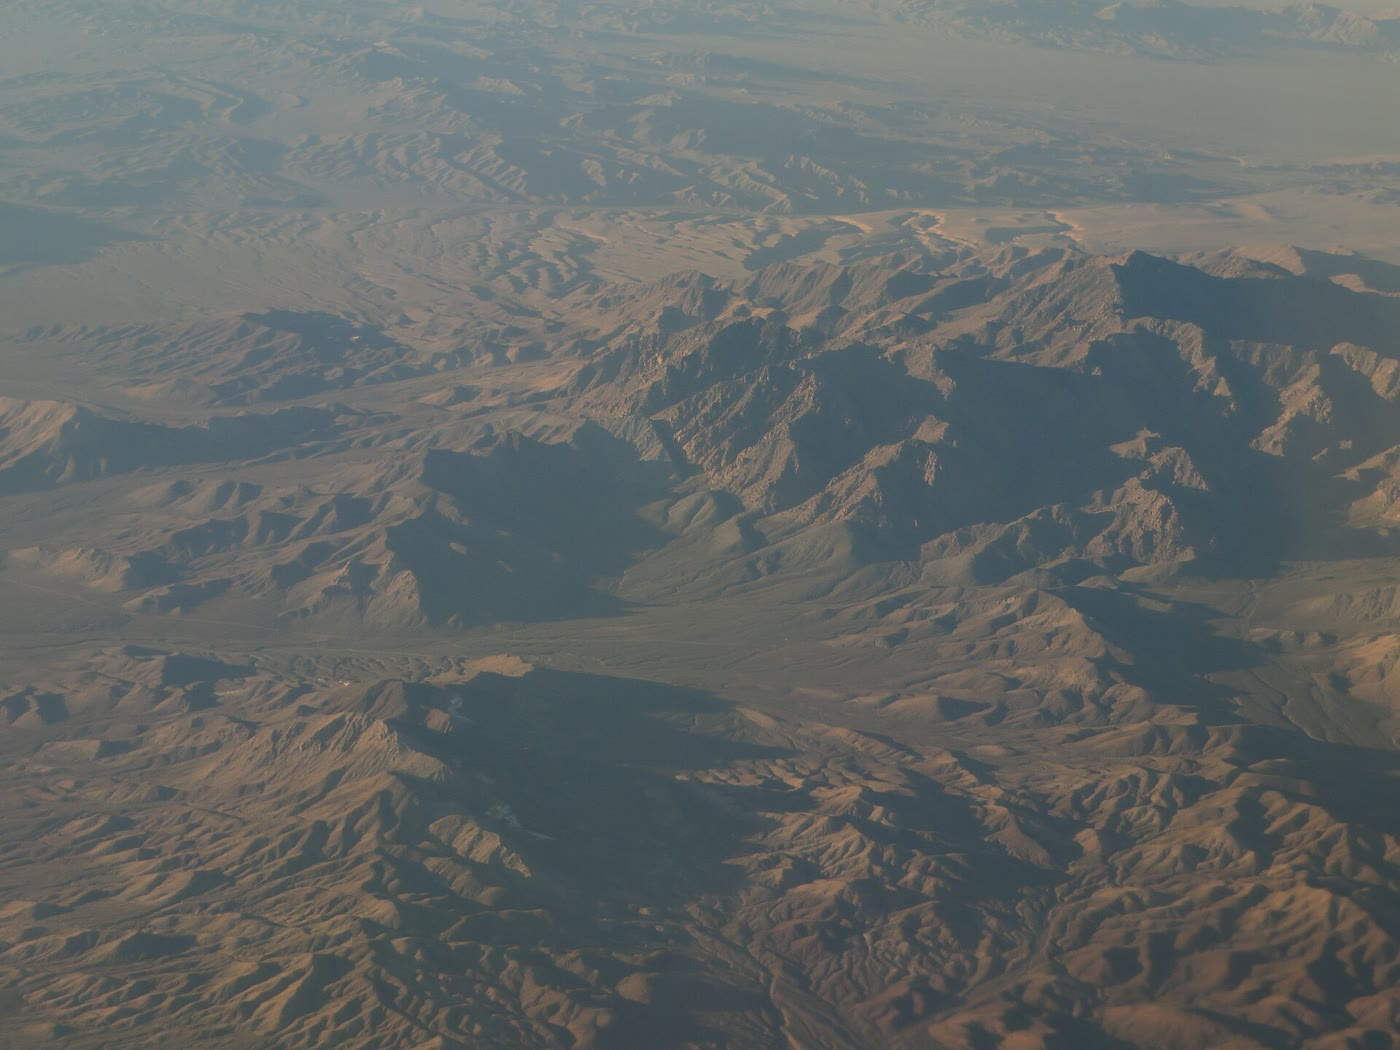
\includegraphics[width=\linewidth]{images/book5/b3-basin-and-range.jpg}

{\scriptsize 加利福尼亚州死谷以南的盆岭地形（航拍）：
平行排列的倾斜断块山脉，由充填沉积物的盆地所分隔。
照片：Ken Lund, CC BY-SA 2.0。}
\end{minipage}
\end{inthefield}
% ledger: photo:b3-basin-and-range

\section{练习}

\begin{exercise}[$\star$]\label{exo:b3:extension-strike-slip:1}
在一个刚性多米诺块体区域中，断层现倾角为 \ang{35}，它们形成时
倾角为 \ang{50}。计算岩层的倾角及伸展因子。
\end{exercise}

\begin{exercise}[$\star$]\label{exo:b3:extension-strike-slip:2}
判断下列每种情形中的阶区是张开成盆地还是抬升成脊，并说明理由：右行断层的右阶；
右行断层的左阶；左行断层的左阶；
左行断层的右阶。
\end{exercise}

\begin{exercise}[$\star$]\label{exo:b3:extension-strike-slip:3}
死海转换断层在约 \qty{20}{Ma} 内移动了 \qty{105}{km}。
计算其平均速率（以 \unit{mm/\text{年}} 计），并与
死海盆地所用的 \qty{6}{mm/\text{年}} 相比较。
\end{exercise}

\begin{exercise}[$\star$]\label{exo:b3:extension-strike-slip:4}
在盆岭省中部，\qty{235}{km} 的伸展量达到
\qty{200}{\percent}。计算该区域伸展前后的宽度，
对伸展量为 \qty{50}{\percent} 的北部，做同样的计算。
\end{exercise}

\begin{exercise}[$\star\star$]\label{exo:b3:extension-strike-slip:5}
圣安德烈亚斯断层在 15 至
\qty{20}{Ma} 内至少移动了 \qty{563}{km}。计算平均速率的范围，并与
现今约 \qty{51}{mm/\text{年}} 的漂移速率相比较。什么因素可以解释二者的差异？
\end{exercise}

\begin{exercise}[$\star\star$]\label{exo:b3:extension-strike-slip:6}
取 $\mu = 0.6$，计算使倾角分别为 \ang{60}、\ang{50} 和 \ang{40} 的
正断层发生滑动所需的\omterm{def:b3:structural-analysis:palaeostress}{应力比} $\sigma_1/\sigma_3$，并求闭锁倾角。
\end{exercise}

\begin{exercise}[$\star\star$]\label{exo:b3:extension-strike-slip:7}
计算正断层在 $\mu = 0.4$ 和 $\mu = 0.2$ 时的闭锁倾角。
需要多大的摩擦系数，才能使倾角为 \ang{15} 的断层
在竖直方向的 $\sigma_1$ 作用下发生滑动？
\end{exercise}

\begin{exercise}[$\star\star$]\label{exo:b3:extension-strike-slip:8}
在平行于滑动方向的地震剖面上，一条\omterm{def:b3:extension-strike-slip:detachment}{铲形断层}的水平断距为
\qty{2.5}{km}；它在 \qty{4.0}{km} 深处变平，成为\omterm{def:b3:extension-strike-slip:detachment}{拆离断层}。
计算位于原上盘顶面之下的洼陷面积，以及位于
深度首次达 \qty{1.5}{km} 的岩层之下的洼陷面积。
\end{exercise}

\begin{exercise}[$\star\star$]\label{exo:b3:extension-strike-slip:9}
死海盆地长 \qty{132}{km}，沿其轴向的伸展系数为
1.19。求其初始长度与伸展量，以及
以 \qty{6}{mm/\text{年}} 的速率伸展所需的时间。
\end{exercise}

\begin{exercise}[$\star\star\star$]\label{exo:b3:extension-strike-slip:10}
断块之间相距 \qty{3.0}{km}（沿垂直于断层的方向量取），
其断层倾角由 \ang{60} 旋转至 \ang{45}。求每个断块在旋转前后的水平宽度、
每个断块的伸展量，以及岩层的倾角。
为什么岩层的倾向必须与断层相反？
\end{exercise}

\begin{exercise}[$\star\star\star$]\label{exo:b3:extension-strike-slip:11}
求 R 与 R$'$ 剪切及张性裂隙的夹角，
设岩石 $\phi = \ang{40}$，\omterm{def:b3:deformation-mechanisms:shear-zone}{剪切带}走向东西、为左行，
以方位角表示，并给出各自的滑动方向。
\end{exercise}

\begin{exercise}[$\star\star\star$]\label{exo:b3:extension-strike-slip:12}
一个由多米诺式断块组成的区域，其断层以最利于滑动的倾角形成，
并不断旋转直至断层闭锁。求仅由旋转所能给出的最大伸展系数，
分别取 $\mu = 0.6$ 与 $\mu = 0.85$，
并说明哪些岩石在必须形成新断层之前还能进一步伸展。
\end{exercise}

\section{问题：梅罗半地堑}

\begin{problem}[{周末问题——虚构裂谷边界的伸展，由其多米诺断块、
铲形断层、变质核杂岩与
调节断层推断}]
\label{pb:b3:extension-strike-slip:1}
% values: calc/ch09.py; domino_extension.py; rollover.py
梅罗半地堑是位于大陆裂谷边缘的一个虚构盆地。
其主断层为\omterm{def:b3:extension-strike-slip:detachment}{铲形断层}，地表处倾角为 \ang{60}。其上盘中
一块宽 \qty{24.0}{km} 的区域被平面断层切割，这些断层现倾向东，
倾角为 \ang{42}，其间岩层向西倾，倾角为 \ang{18}。在平行于滑动方向的地震剖面上，
主断层的水平断距为 \qty{3.2}{km}，且其上盘顶面
低于原始水平面，形成的洼陷面积为
\qty{16.0}{km^2}。沿走向向南，剥蚀已移除同一体系的上盘，
并暴露出一个\omterm{def:b3:extension-strike-slip:core-complex}{变质核杂岩}。向北，一条
左行调节断层将该半地堑与下一个半地堑相连。取 $\mu =
0.6$，$g = \qty{9.8}{m/s^2}$，地壳密度为
\qty{2800}{kg/m^3}。

\medskip\noindent\textbf{第一部分——多米诺断块。}
\begin{enumerate}
  \item 为什么断层的初始倾角等于现今断层倾角与岩层
        倾角之和？给出该值，并将其与安德森理论作比较。
  \item 求该区域的伸展系数。
  \item 求其初始宽度及其所记录的伸展量。
  \item 求使断层现在发生滑动所需的比值 $\sigma_1/\sigma_3$，
        并将其与取向良好的新断层的比值作比较。
  \item 这些断层在何种倾角下闭锁，区域仅靠旋转能达到
        怎样的伸展系数？此后会发生什么？
\end{enumerate}

\medskip\noindent\textbf{第二部分——铲形主断层。}
\begin{enumerate}[resume]
  \item 借助等断距作图法说明，为何上盘岩层
        向断层倾斜。
  \item 求\omterm{def:b3:extension-strike-slip:detachment}{拆离断层}的深度。
  \item 已知洼陷面积的精度为 \qty{10}{\percent}，深度的
        确定程度如何？
  \item 对于首次深达 \qty{2.0}{km} 的岩层，
        预测其洼陷面积。
  \item 穿过主断层的水平伸展量是多少？
  \item 半地堑的沉积物如何记录断层的
        活动？
\end{enumerate}

\medskip\noindent\textbf{第三部分——核杂岩。}
\begin{enumerate}[resume]
  \item 下盘糜棱岩在 \qty{5.5}{kbar} 下达到平衡，求其
        深度。
  \item 其云母在 \qty{24}{Ma} 时对氩封闭，同一糜棱岩的卵石
        出现在半地堑充填物中，时间为 \qty{16}{Ma}。求
        平均折返速率，并取封闭深度等于
        上一问所求的深度。
  \item 要使糜棱岩折返至地表，\omterm{def:b3:extension-strike-slip:detachment}{拆离断层}上需要多大的滑移量，
        若其平均倾角为 \ang{30}，水平伸展量又为多少？
  \item 该\omterm{def:b3:extension-strike-slip:detachment}{拆离断层}今日在地表的倾角为 \ang{15}。它能否在竖直方向
        的 $\sigma_1$ 作用下以该倾角滑动？请给出两种解决途径。
  \item 若其在深部以 \ang{45} 滑动，出露部分
        转过了多大角度？原因何在？
  \item 比较\omterm{def:b3:extension-strike-slip:core-complex}{变质核杂岩}的伸展量与
        半地堑的伸展量。
\end{enumerate}

\medskip\noindent\textbf{第四部分——调节断层。}
\begin{enumerate}[resume]
  \item 左行调节断层向左阶移 \qty{4.0}{km}，其两条
        断层分支重叠达 \qty{3.0}{km}。该阶移会张开盆地，
        还是抬升成脊？
  \item 该断层以 \qty{5}{mm/\text{年}} 的速率滑动了 \qty{1.2}{Ma}。求
        其位移量。
  \item 求张开的面积、盆地底面的长度（重叠量加
        位移量）及其长与宽之比。
  \item 将该比值与死海盆地的比值作比较，死海盆地长 \qty{132}{km}，宽 7
        至 \qty{10}{km}。
  \item 若同一断层向相反方向弯曲，会形成什么构造，
        穿过它的剖面将显示什么？
  \item 梅罗半地堑的水平伸展总量是多少，
        包括主断层与多米诺断块的贡献？
\end{enumerate}
\end{problem}
